\documentclass[a4paper,12pt]{article}

\sloppy
\frenchspacing

\usepackage[left=4cm,top=4cm,right=4cm,bottom=4cm,nohead]{geometry}
\usepackage[utf8]{inputenc}
\usepackage[magyar]{babel}
\usepackage{listings}
\usepackage{multicol}
\usepackage{graphicx}
\usepackage{float}

\title{Szoftverarchitektúrák (VIAUM105)\\Egyszerű verziókövető rendszer\\Rendszerterv}
\author{Vajna Miklós (AYU9RZ)\\Veres-Szentkirályi András (YZIOAW)}

\begin{document}

\maketitle
\thispagestyle{empty}
\lstset{numbers=left, numberstyle=\tiny, basicstyle=\ttfamily, breaklines=true, frame=single, tabsize=2}

\pagebreak
\onehalfspacing
\section{Bevezetés}

Jelen rendszerterv célja a házi feladat tervezése során meghozott döntések
dokumentálása. A döntéseket két csoportra oszthatjuk:

\begin{itemize}
\item architektúrával kapcsolatos döntések
\item az egyes rétegekkel kapcsolatos döntések
\end{itemize}

\section{Architektúra}

A rendszert 3 réteg alkotja:

\begin{figure}[H]
\centering
\includegraphics[width=25mm,keepaspectratio]{layers.png}
\caption{A verziókövető rendszer architektúrája}
\end{figure}

\begin{itemize}
\item Adatbázis réteg: SQL adatbázis az entitások permanens tárolására.
\item Kiszolgáló: itt kerül implementálásra az üzleti logika, tehát minden
olyan funkcionalitás, mely nem triviális, és megjelenítés-független.
\item Kliens: a megjelenítési rétegért felel, csak triviális funkciókat
tartalmaz, minden egyéb funkciót a kiszolgálón keresztül biztosít.
\end{itemize}

\section{Adatbázis réteg}

Fizikailag a következő entitásokat kívánunk tárolni:

\begin{itemize}
\item a rendszer felhasználóit
\item a modelleket
\item a modellek egyes verzióit
\item a modellekhez való hozzáférési jogokat
\end{itemize}

\begin{figure}[H]
\centering
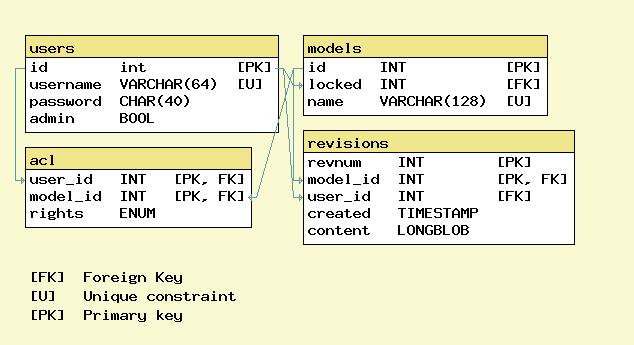
\includegraphics[width=120mm,keepaspectratio]{sqlschema.png}
\caption{Az adatbázis sémájának modellje}
\end{figure}

Az ábrán látható módon ezek között a következő kapcsolatokat tervezzük:

\begin{itemize}
\item a felhasználók és modellek között jogosultságokat adhatunk meg
\item a felhasználók zárolhatják a modelleket
\item a modellekhez egy-egy felhasználó verziókat hozhat létre
\end{itemize}

\section{Üzleti logika}

FIXME ide johetne corba interfeszrol class diagram, lehetne dumalni az sql
injection elleni prepared statementekrol, tie megoldasokrol

\section{Megjelenítési réteg}

FIXME

\section{Befejezés}

FIXME

\section{Továbbfejlesztési lehetőségek}

FIXME itt lehetne reszletezni az omniorb vs ssl kerdest, addig is vpnt ajanlani

\end{document}
